\documentclass{article}
\usepackage[utf8]{inputenc}
\usepackage[a4paper, total={6in, 8in}]{geometry}

\vspace{4in}
\title{CSCI4998 Final Year Project I\\Oculus Rift Project\thanks{Supervised by Professor Jiaya Jia}}
\author{IP Wing Ha (1155033071)\\YUNG Man Lee (1155032377)}
\date{2 December 2015}

\usepackage{natbib}
\usepackage{graphicx}
\usepackage{caption}
\usepackage{subcaption}
\usepackage{calc}
\usepackage{url}
\usepackage[none]{hyphenat}%%%%
\usepackage{pgfgantt}
\usepackage{pdflscape}

\setlength{\parindent}{0pt}

\begin{document}

\begin{titlepage}
	\centering
	%\includegraphics[width=0.15\textwidth]{example-image-1x1}\par\vspace{1cm}
	{\scshape\LARGE The Chinese University of Hong Kong\par}
	\vspace{1cm}
	{\scshape\Large {CSCI4998 Final Year Project I} \par}
	\vspace{1.5cm}
	{\huge\bfseries {Oculus Rift Project} \par}
	\vspace{2cm}
	{\Large\itshape IP Wing Ha (1155033071)\\YUNG Man Lee (1155032377)\par}
	\vfill
	supervised by\par
	Professor Jiaya \textsc{Jia}

	\vfill

% Bottom of the page
	{\large \today\par}
\end{titlepage}

\setcounter{tocdepth}{2}
\tableofcontents

\clearpage

\section{Introduction}
Virtual reality (VR) has become a big trend in gaming industry. A game in virtual world can make player have more interactive and funny experience. A horror VR game can provide an exciting and terrified game experience without causing danger in real life.\\ \\
This project is a VR horror game develop for Oculus Rift, which is supported by multiple OS on PC.
\begin{figure}[h!]
\centering
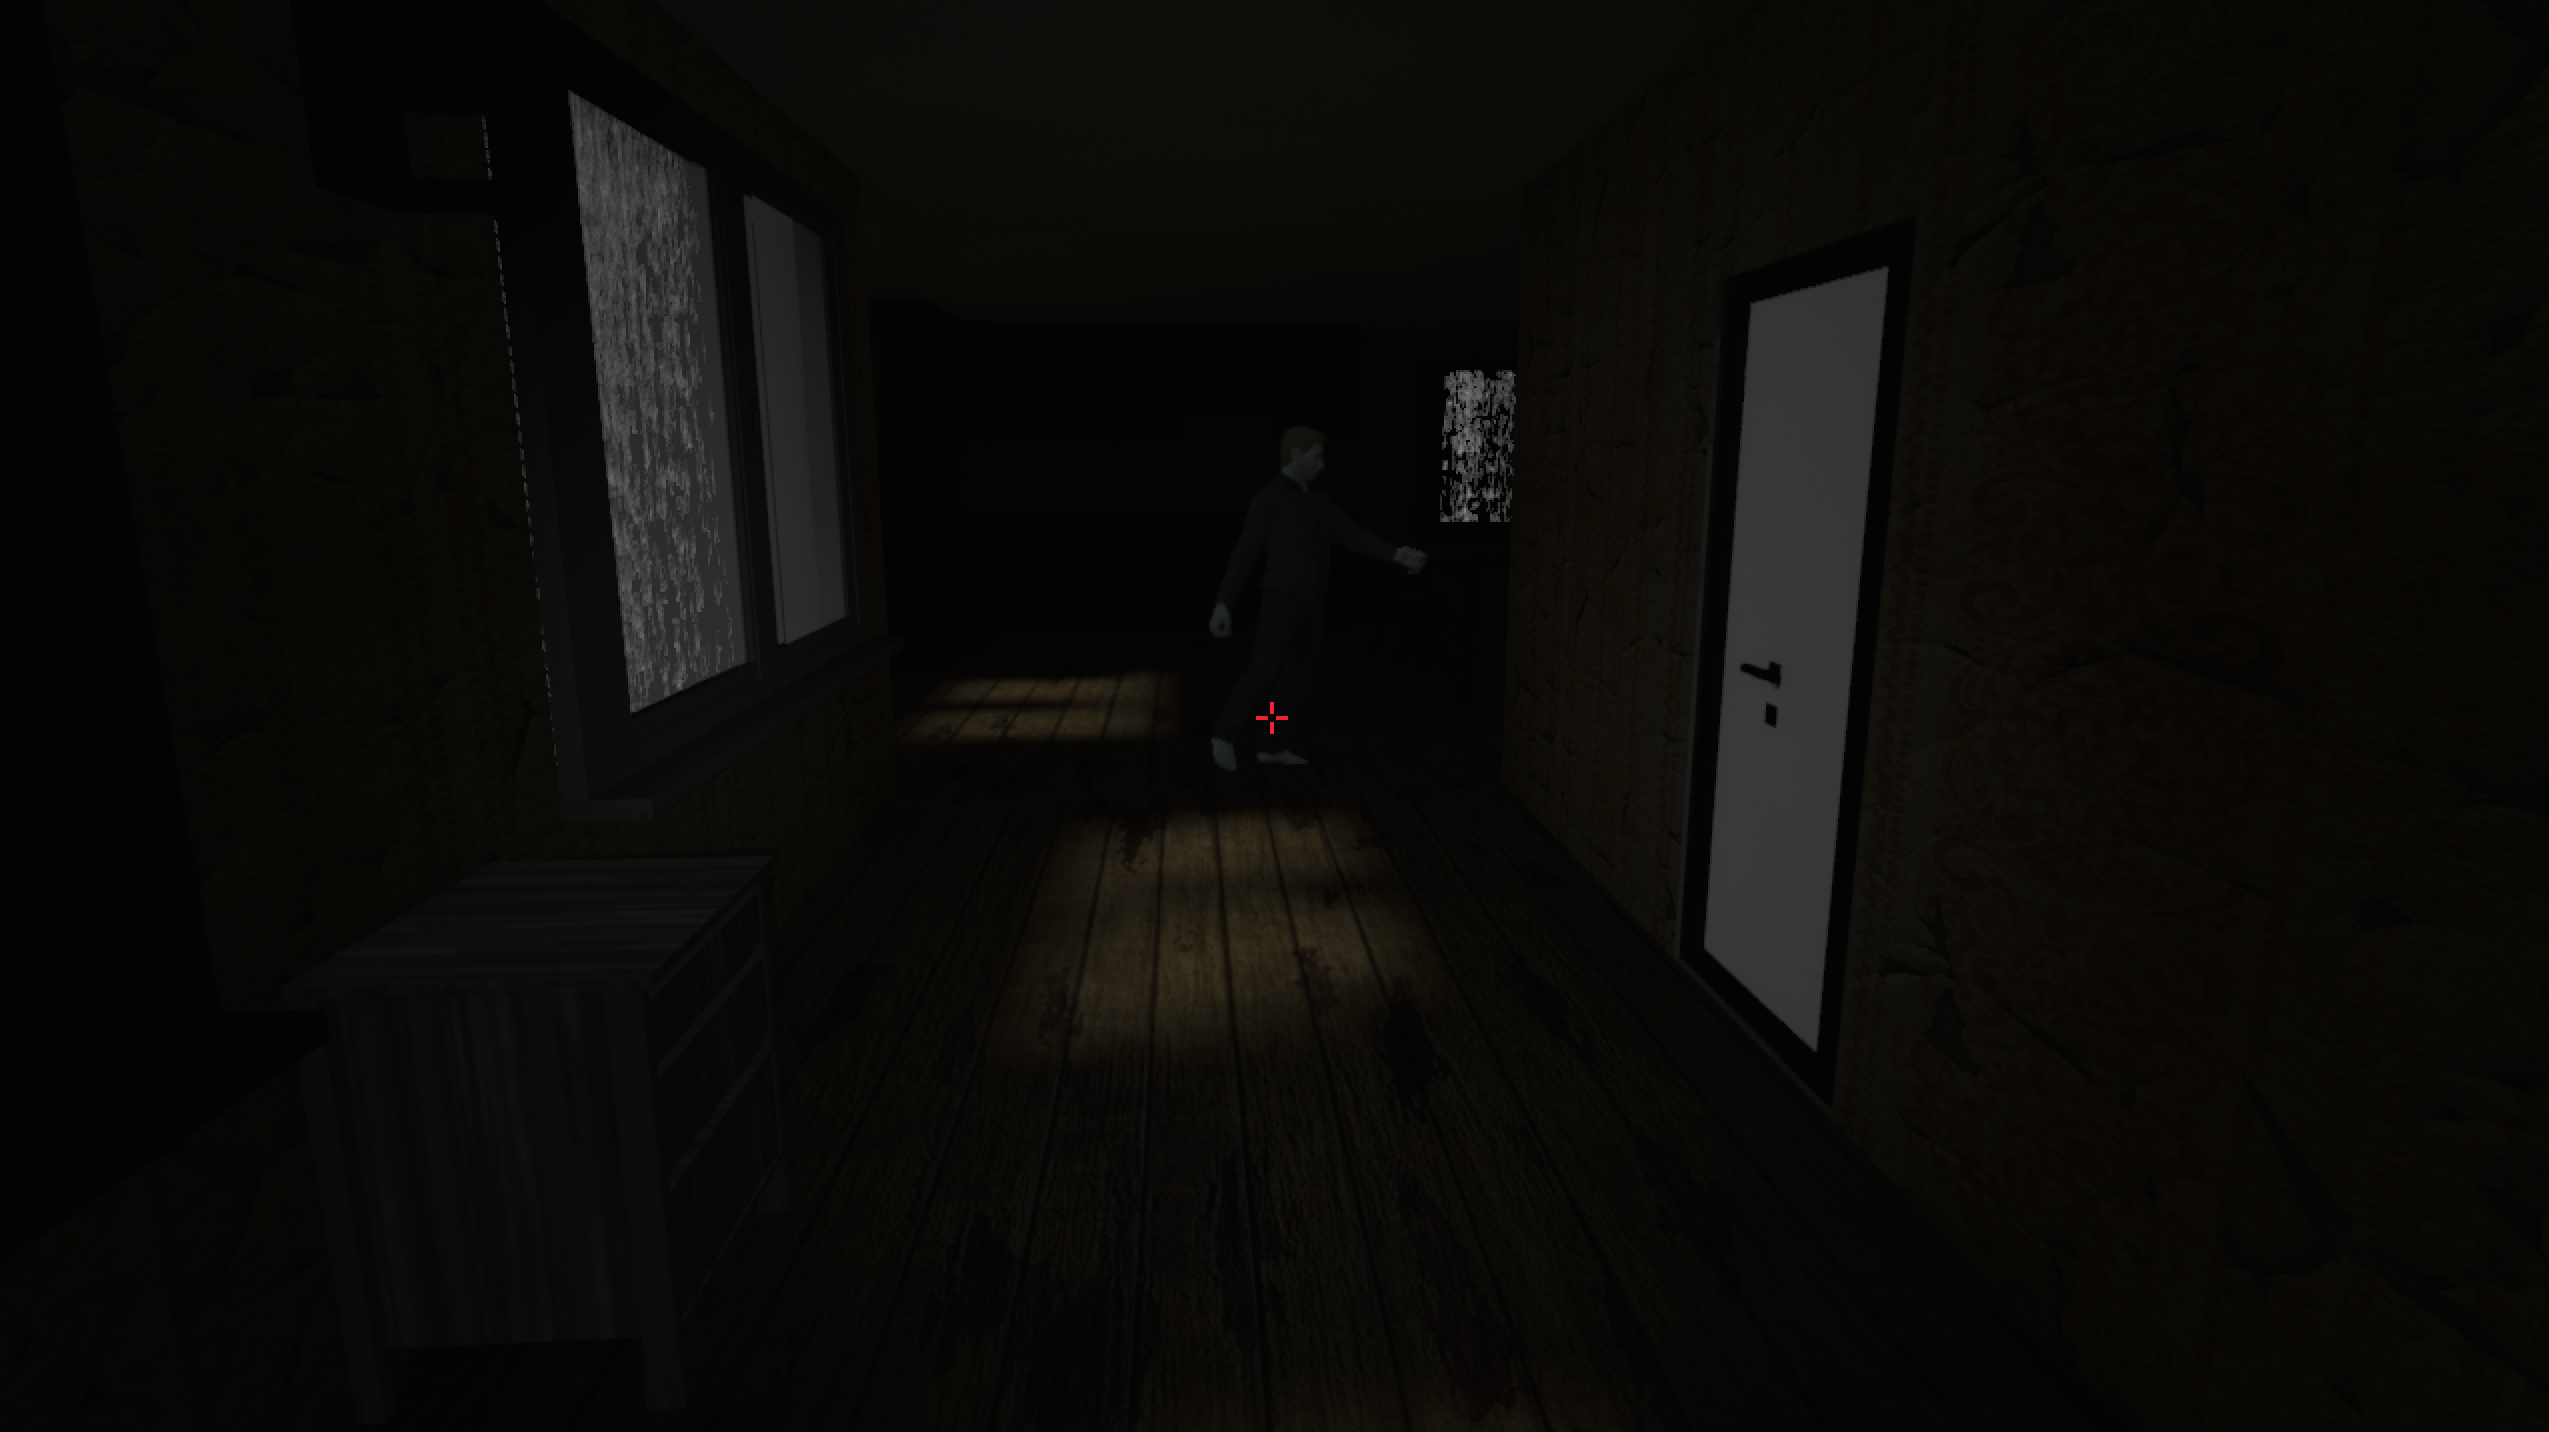
\includegraphics[width=\textwidth]{gamecapture.png}
\caption{Screen capture of the game}
\label{fig:gamecapture}
\end{figure}

\bigskip

\subsection{Motivation}
A good game should provide not only with the function. The more important is the game progress should be enjoyable.\\This project aims to provide an exciting and enjoyable experience to every player, where the traditional final year project may not consider.\\ \\
From the prospective of a professional software engineer, computer game project emphases on software developing cycle, graphics, scripting and animation. Integrating software knowledge with good use of media is a breakthrough for computer science students.

\clearpage

\section{Milestones}
This project started in August, with topic "Continue on the cardboard glasses (CSCI3290) (Team 2)". In early October, the project is changed to an Oculus project after taken careful considerations.
\subsection{Time line}
Below is the detailed time line of the major changes of our project:
%\smallskip
\begin{center}
  \begin{tabular}{ l | p{12cm} }
    August 2015 & Topic brainstorming and decided to work on Horror Game \\
     & \\
    September 2015 & Tried developing the game via Unity and Cardboard SDK.  \\
     & Planned and decided the story settings \\
     & \\
    Early October 2015 & Took supervisor\textsc{\char13}s suggestion and developed the game for Oculus \\
     & Restarted the project on Unreal Engine 4 \\
      & \\
    October 2015 & Built and made events for the living room \\
     & \\
    November 2015 & Built and made events for the corridor and the lumber room \\ 
     & \\
    Late November 2015 & Reviewed the whole project \\
     & Testing and fine-tuning the game design
  \end{tabular}
\end{center}

\subsection{Gantt Chart}
The Gantt Chart shows the relations between the events and a clearer view of the time line in weekly format (Refer to Appendix A).

\clearpage

\section{Research on the hardware and software used}
\subsection{Comparison between Google Cardboard and Oculus Rift}
Google Cardboard\citep{cardboard} and Oculus Rift\citep{oculus} are very common in building VR applications. In August, this project developed based on Google Cardboard. After one month, we found that there are a lot of drawbacks using Google Cardboard.

\begin{center}
  \begin{tabular}{ | p{2cm} | p{6cm} | p{6cm} |}
    \hline
     & \textbf{Google Cardboard} & \textbf{Oculus Rift Development Kit 1} \\ \hline
    Head movement control & Depends on the mobile phone, usually has more sensors than Oculus Rift & Gyroscope, Accelerometer and Magnetometer\\ \hline
    Input Control & Limited to one button & Can connect to computer, joystick and game controller \\ \hline
    Cost & {Cardboard can be hand made with very low cost \hfill} & For Development Kit 1 (DK1): About HK\$ 2500 \\ \hline
    Software support & Android and Unity SDK & PC, Mobile and Audio SDK, including Unreal Engine and Unity Integration \\ \hline
    Screen resolution & Depends on the resolution of the phone. It looks blurred and pixelated when magnify by Google Cardboard & 1280 x 800 for Oculus DK1 \\ \hline
    Portability & No standard device set, application must deal with different devices & Support multiple platforms (Windows, Mac and Linux) \\ \hline
    Flexibility & Can work independently without the computer & Must work with PC \\ \hline
    Computation & Limited by the specification of mobile phone used & Depends on the computer, which is much higher than mobile phone \\
    \hline
    Battery life & Consume a lot of power when running VR application & Depends on the computer, usually 5 hours onwards \\
    \hline
  \end{tabular}
\end{center}
\smallskip
When we tested to develop on mobile phone, the screen resolution is very low and the image cannot be seen clearly. The control is limited to the single button of the cardboard. In addition, the device get hot very easily and the battery drops rapidly. As a result, we took supervisor\textsc{\char13}s suggestions and switched to developing with Oculus Rift Development Kit 1 (DK1).
\smallskip
\begin{figure}[hp!]
    \centering
    \begin{subfigure}[b]{0.3\textwidth}
        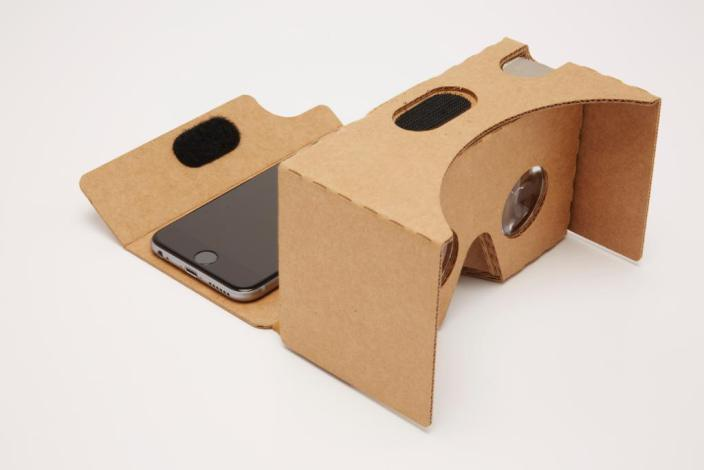
\includegraphics[width=\textwidth]{Cardboard}
        \caption{Google Cardboard}
        \label{fig:Cardboard}
    \end{subfigure}
    \begin{subfigure}[b]{0.3\textwidth}
        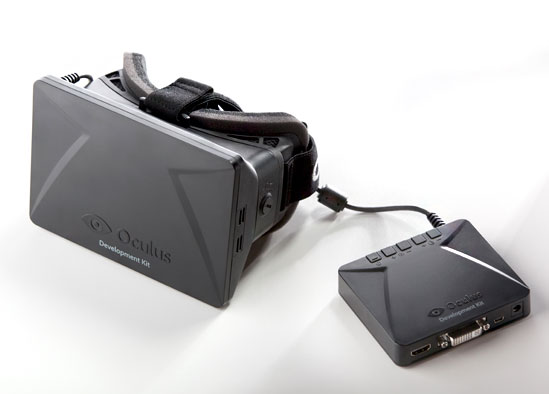
\includegraphics[width=\textwidth]{oculusdk1}
        \caption{Oculus Rift DK 1}
        \label{fig:oculusdk1}
    \end{subfigure}
    \caption{Pictures of the common VR devices}\label{fig:devices}
\end{figure}

\clearpage

\subsection{Comparison between Unity and Unreal Engine}
Unity and Unreal Engine are two game engines that commonly used in game development. After having game development experience on both of them, a conclusion is drawn: \smallskip
\begin{center}
\begin{tabular}{ | p{2cm} | p{6cm} | p{6cm} | }
 \hline
 & \textbf{Unity 5 (Free Version)} & \textbf{Unreal Engine 4} \\
 \hline
 \textbf{Price} & Free & Free since March 2015 \\
 \hline
 \textbf{Function} & Limited, for example: no mirror effect & Powerful, for example: has eye lighting adaptation \\
 \hline
  \textbf{Version Control} & The project size is very large and it exceeds the upper size limit when committing to Git. Unity provide their own version control tool but it is unavailable in free version & Project size is relatively smaller and customized version control setting is available \\
 \hline
 \textbf{Level of Difficulty for Beginners} & Low. Easy to get started. & High. A lot of functions and parameters are needed to be tuned. \\
 \hline
 \textbf{Supported VR Devices} & Oculus Rift, Gear VR, Playstation VR, Google Cardboard & Oculus Rift, Gear VR, PlayStation VR, HTC Vive, Steam VR (Official news has mentioned that Google Cardboard will be supported in the future) \\
 \hline
 \textbf{Royalty fee} & None & 5\% on gross revenue after earning US\$3000 per product\citep{royalty} \\
 \hline
\end{tabular}
\end{center}
\bigskip
Unreal Engine is picked due to powerful functionality and embedded version control. As it is very important to keep the project shared and version controlling, we decided to move the project to Unity when switching the project from Google Cardboard project to Oculus Rift project.
\newpage

\section{Game Design \& Development}
\subsection{Story}
The player was watching TV in her house at a rainy night. Suddenly, the light went out but she managed to find a flashlight. She stepped out of the living room and discovered the room was connected to another world.\\ \\
After a few horror events, the player found out that she is in a bloody house with a girl Dora and Dora\textsc{\char13}s father, where a murder has taken place.\\

\subsection{Architecture}
Figure \ref{fig:ArchitectureDiagram} shows the architecture  of the game. The game executable can be run on PC. It is required to connect the Oculus and the PC with USB and HDMI to detect the head movement and showing the output screen. Player can choose to use keyboard or gaming controller to control the movement in game.
\bigskip
\begin{figure}[hp!]
\centering
\includegraphics[width=0.9\textwidth]{ArchitectureDiagram.png}
\caption{Architecture Diagram of this game}
\label{fig:ArchitectureDiagram}
\end{figure}

\newpage
\subsection{Game Logic}
In this semester, the game is separated into three stages.\\
In the first stage, the scene take place in the living room. Due to a power cut, the player need to find the flashlight to leave the room. After leaving the room, the player entered the corridor and there is no way to get back to the living room. Player need to find a key to get in the lumber room and enter the third stage, where the player is locked in the room and needed to get more clues of the story. After that, the player would have more ideas about the story. \par
\bigskip
\begin{figure}[hp!]
\centering
\includegraphics[width=0.25\textwidth]{FYP_Overview.png}
\caption{Overview of the game logic}
\label{fig:FYP_Overview}
\end{figure}
\clearpage

\subsubsection{First stage - Events in Living Room}
The first stage begins with a rainy and stormy night. The player is sitting on sofa and watching television. Walking control is disabled but head movement is allowed. After 10 seconds, all lights go out due to a power cut. The player can start exploring the room with interactive events (Refer to Figure \ref{fig:FYP_FirstScene}). \par
\bigskip

\begin{figure}[hp!]
\centering
\includegraphics[width=\textwidth]{FYP_FirstScene.png}
\caption{State Machine Diagram of the events in living room}
\label{fig:FYP_FirstScene}
\end{figure}

\clearpage
\subsubsection{Second stage - Events in corridor}
After leaving the living room, the player entered a corridor which is not her original house. She went to another world and the door connected has disappeared. After some horror events, she can find the key and get in to the lumber room. (Refer to Figure \ref{fig:FYP_SecondScene})\par
\bigskip

\begin{figure}[hp!]
\centering
\includegraphics[width=\textwidth]{FYP_SecondScene.png}
\caption{State Machine Diagram of the events in corridor}
\label{fig:FYP_SecondScene}
\end{figure}

\clearpage
\subsubsection{Third stage - Events in lumber room and afterwards}
When the player entered the lumber room, the door is locked and the player cannot leave the room. There is some arguing sound outside the room. After peeking outside, the door is unlocked (Refer to Figure \ref{fig:FYP_ThirdScene}). The player can explore the changes of the corridor and explore more about the story. \par
\bigskip
\begin{figure}[hp!]
\centering
\includegraphics[width=\textwidth]{FYP_ThirdScene.png}
\caption{State Machine Diagram of the events in lumber room}
\label{fig:FYP_ThirdScene}
\end{figure}
\clearpage

\subsection{Lighting}
There are 4 types of light available in Unreal Engine. Three of them are used in the game.

\subsubsection{Directional Light}
Light that emits from infinitely far can be simulated by using directional light. It is a suitable choice for simulating sunlight or moonlight. Unlike other types of light, the shadow created will not be affected by the distance between the object and the light source. The shadow is always parallel. \\

\begin{figure}[hp!]
\centering
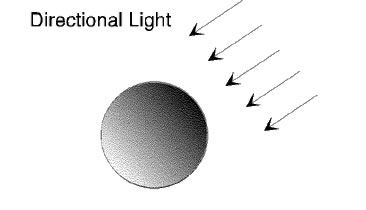
\includegraphics[scale=0.6]{directional_light.jpg}
\caption{Directional Light}
\label{fig:directional_light}
\end{figure}
\smallskip

In the game, moonlight is simulated by using this lighting type. Also, the environmental lighting is heavily depended on it. As light in real world will bonce between different surfaces, by setting the value of indirect light, indoor area is still lighted up even if there is no direct lighting.\\ 
\begin{figure}[hp!]
\centering
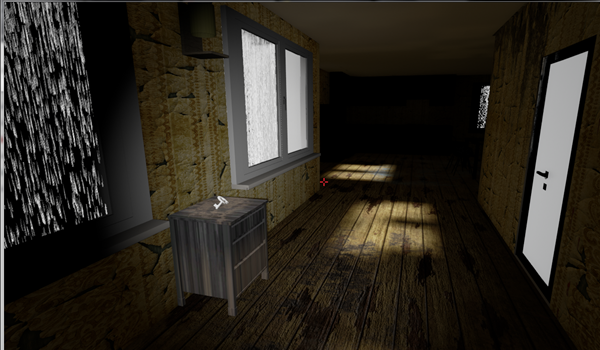
\includegraphics[scale=0.6]{moonlight.png}
\caption{Moonlight}
\label{fig:moonlight}
\end{figure}

\clearpage

\subsubsection{Spot Light}
Light that emits from a point in a cone shape can be simulated by using spot light. It is very suitable for simulating stage light or light in disco. \\
\begin{figure}[hp!]
\centering
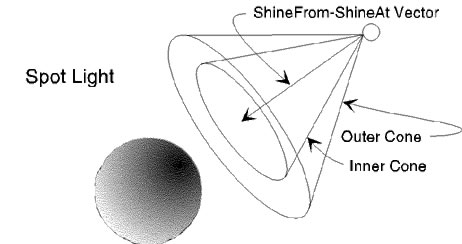
\includegraphics[scale=0.6]{spot_light.jpg}
\caption{Spot Light}
\label{fig:spot_light}
\end{figure}
 \\ \\
In the game, the light from flashlight is simulated by using this lighting type. \\
\begin{figure}[hp!]
\centering
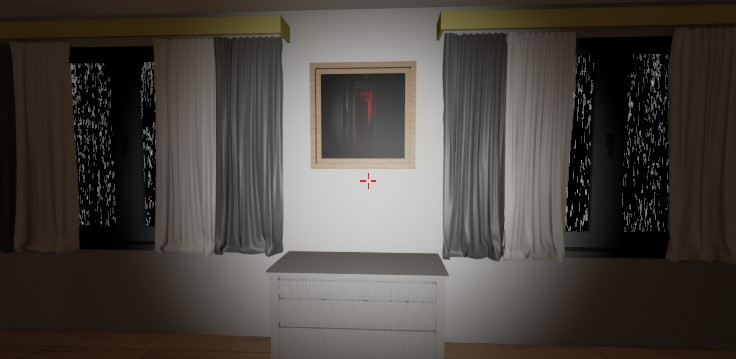
\includegraphics[scale=0.6]{spotLight1.jpg}
\caption{Light from flashlight}
\label{fig:spot_light1}
\end{figure}
\clearpage
\subsubsection{Point Light}
Light that emits from a point equally in all direction and in sphere space  can be simulated by using spot light.
\bigskip
\begin{figure}[hp!]
\centering
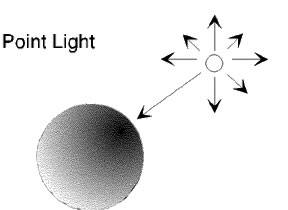
\includegraphics[scale=0.6]{point_light.jpg}
\caption{Point Light}
\label{fig:spot_light1}
\end{figure}
In the game, the light from light bulb is simulated by using this lighting type.
\bigskip
\begin{figure}[hp!]
\centering
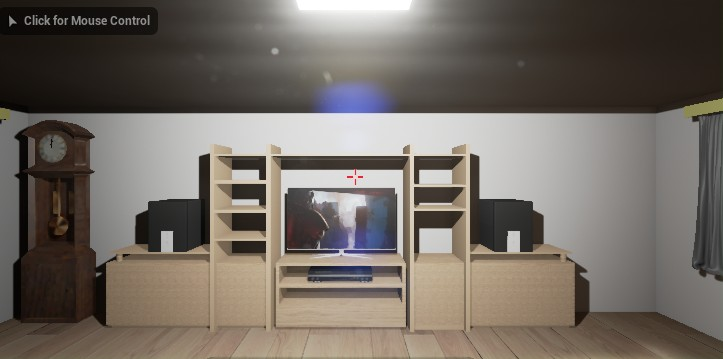
\includegraphics[scale=0.6]{pointLight1.jpg}
\caption{Light bulb}
\label{fig:spot_light1}
\end{figure}

\clearpage
\subsection{Material}
In order to make the object looks more realistic, material is another important component to handle.\\

\subsubsection{Surface}
 \begin{tabular}{ | p{2cm} | p{12cm} | }
 \hline
 \textbf{Parameter} & \textbf{Usage in the game} \\ 
 \hline
 Base Color & Color of the material. Texture image can also be used to connect this node. For special materials like wall paper or floor, seamless texture images are usually used. For more complicated objects, a texture map can be used. \\ 
 \hline
 Metallic & The value is set to 0 for most of the materials unless it is a metal object like the flashlight in the game. \\
 \hline
 Specular & Some materials can be a little reflective but it is not a metal. For example, materials such as waxed wood floor will have a high value. \\
 \hline
 Roughness & The value is set higher for matte materials. \\
 \hline
 Emissive Color & The value decides the color that emits from the material and the level of its brightness. The parameter is kept unchanged for most of the materials except the materials of light sources such as lamp. \\
 \hline
 Opacity & The value is useful for creating transparent materials such as glass. \\
 \hline
 Opacity Mask & The alpha channel is connected to this node when the texture image is partly transparent. \\
 \hline
 Normal & A normal map can be connected if the material’s surface is bumpy. \\
 \hline
\end{tabular}
\bigskip

Here is an example of the material of a wooden floor (the floor of living room). The base color is texture of wood. For metallic, specular and roughness, they are unchanged in this case. Only specular is changed. Also, a normal map is connected to the material so that the junction of the wooden planes on the floor is concave.\\

\begin{figure}[h]
\centering
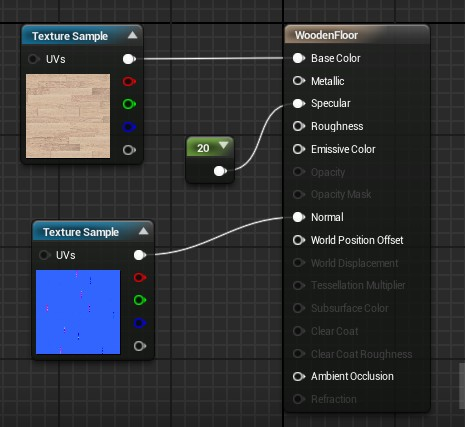
\includegraphics[scale=0.6]{material1.jpg}
\caption{Material of wooden floor}
\label{fig:material1}
\end{figure}

\clearpage

\subsubsection{Deferred Decal}
Deferred decal shares most of the parameters with surface. However, it is used mainly for creating blood trace or splash in the game as it will not simply duplicate its texture on an object’s surface. After setting its normal aligned with the object surface, the material will look like it is being “attached” on the surface of an object or even multiple objects if the area is big enough to cover.\\ \\
\begin{figure}[h]
\centering
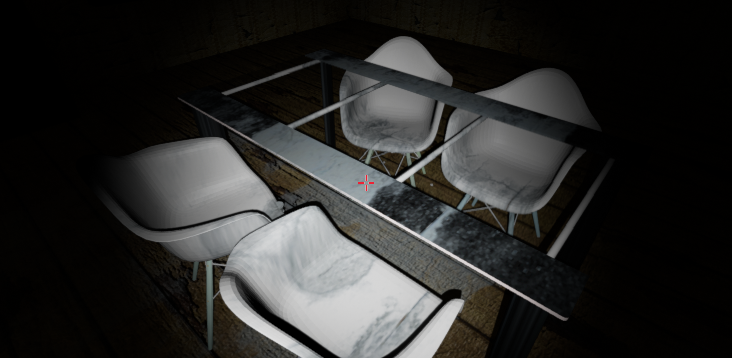
\includegraphics[scale=0.6]{material2.png}
\caption{Dust on the table set}
\label{fig:material2}
\end{figure}

\newpage

\subsection{3D Scene}
Graphics and asset is essential part to game experience.

\subsubsection{Environment}

\begin{enumerate}
    \item \textbf{Building} \\
    As the game is played in indoor areas, the real appearance of the house is not a major part to be considered. Rooms are build by putting cube together to form walls and windows are made by subtracting areas from the wall.
    
    \item \textbf{Particle System} \hfill \\
    A particle system is divided into 4 parts which are Appearance, Initial states, Spawn, Behaviour and Lifetime. \citep{ue4particle} In this game, Rain and lightning use techniques of particle system to simulate their physical properties.
    
    \begin{description} 
        \item[Appearance] \hfill \\
        It is the material applied on particles. It works as a "stamp" and copy the same appearance to newly created particles. Material also affects how light is absolute or reflected by the particles. Different materials have different absorption light spectrum and hence different colors will be displayed.
        
        \item[Initial states] \hfill \\
        Refer to the attributes when a particle is created. For example, the size and the initial velocity of particle.
        
        \item[Spawn] \hfill \\
        Determines how many particles are created by emitter at a certain time and also how fast of the creation. It helps to predict and limit the number of particles at the scene at any time. Setting a upper bound of particle emission is useful when frame per second (FPS) is too low so that the quality and smoothness of the game is greatly affected by numerous particles.
        
        \item[Behaviour] \hfill \\
        Gives the spirit to particles. It defines how the states change along the time and how the particles are affected by environment or even other particles. Common behaviours in a game are gravity, collision, velocity, angular velocity, etc.
        
        \item[Lifetime] \hfill \\
        It is the life cycle of the particles. It determines when a particle will be destroyed. Take rain as example, it will be destroyed at several seconds after falling on the floor.
    \end{description}
\end{enumerate}

\clearpage
\subsubsection{Object}
Most of the 3D objects in the game comes from websites that provide free resources. However, some of them still need to be modified before importing into the project as they may not fit the game perfectly. Basically, only extracting components and re-origination are made on the object. \\ \\ 

\textbf{Extracting} \\

In the game, one of the trigger is about a book dropping from the shelf. The shelf could be imported as a single object into the project but it is impossible to have a book dropping from it. Or it could be imported as a combination of objects (a shelf and a number of books) but this increases the computation time. The better way is to separate the book and, the shelf and rest of the books into two objects. Similar things are done on other objects in the game. \\ \\

\begin{figure}[h]
\centering
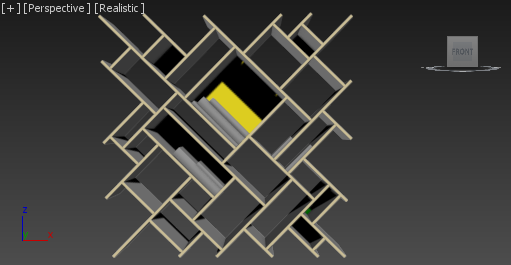
\includegraphics[width=\textwidth]{3dscene1.png}
\caption{Screen capture of the bookshelf in the game}
\label{fig:3dscene1}
\end{figure}
\bigskip

\clearpage
\textbf{Origination} \\

A common drawback of having free assets is their qualities are not guaranteed. They could have unreasonable positioning, like a mile away from the origin.\\

For example, even though this door is centered nicely, it is still not suitable to export in the project. (Refer to Figure \ref{fig:3dscene2})\\

\begin{figure}[h]
\centering
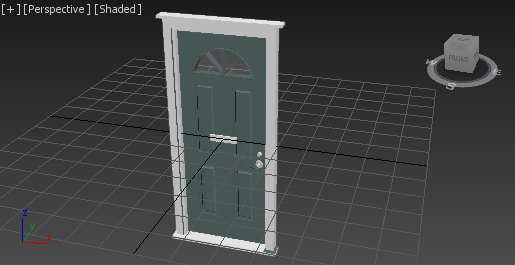
\includegraphics[scale=0.6]{3dscene2.png}
\caption{Door with bad positioning}
\label{fig:3dscene2}
\end{figure}

\smallskip
It is because when the door rotates, it rotates along the z-axis but it is not reasonable in the real world. (Refer to Figure \ref{fig:3dscene3}) Although the issue can be solved by translating the object in game logic each time it rotates, it requires unnecessary resources for calculation in real time. The better way is to make the left side of the door aligning with the z-axis before importing.\\

\begin{figure}[h]
\centering
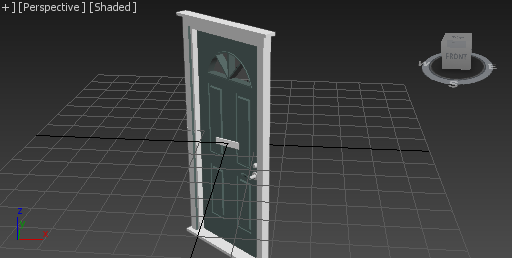
\includegraphics[scale=0.6]{3dscene3.png}
\caption{Door rotation with incorrect z-axis}
\label{fig:3dscene3}
\end{figure}


\clearpage
\subsection{Character and Animation}

\subsubsection{Character}
Again, it is not efficient to model the characters from none. Two software named MakeHuman\citep{MakeHuman} and Fuse\citep{Fuse} are used. They allow users to customize the character them want. No matter a little girl or a old man, the character can be made by turning different parameters easily.

\begin{figure}[h]
\centering
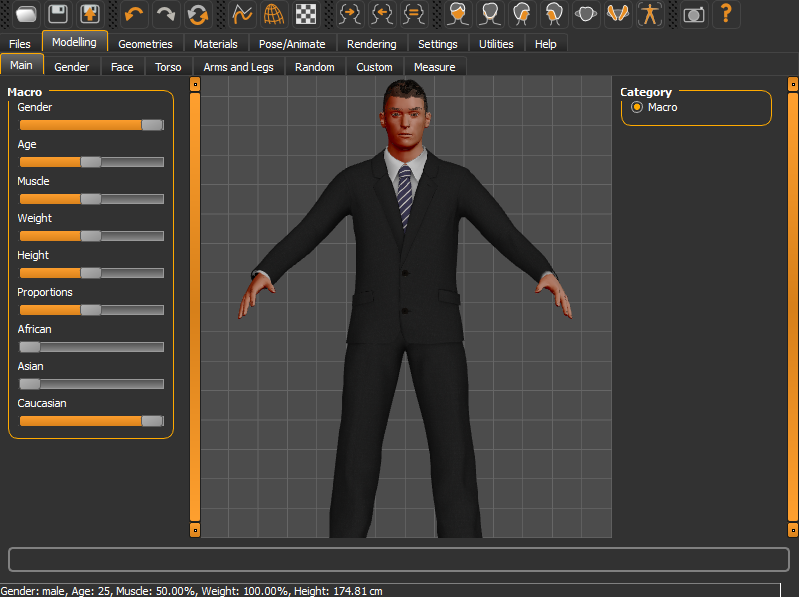
\includegraphics[width=\textwidth]{character1.png}
\caption{Make Human}
\label{fig:character1}
\end{figure}

Another powerful feature of these softwares is the model is rigged automatically. That means the positions of joints or facial features are set already. Only rigged model can be modified to form animation.

\pagebreak

\subsubsection{Animation}
A powerful website named Mixamo\citep{Mixamo} is used to create the animations.

\bigskip

\begin{figure}[h]
\centering
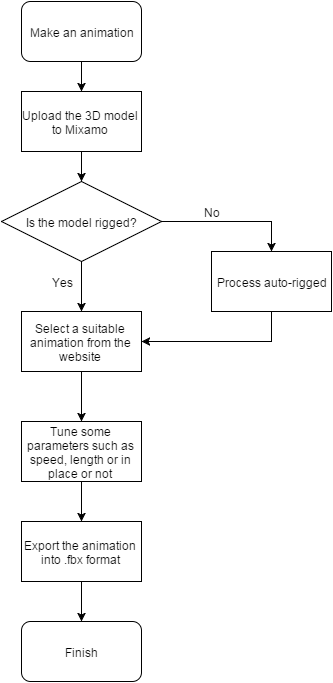
\includegraphics[scale=0.6]{animation1.png}
\caption{Flow chart of creating an animation on Mixamo}
\label{fig:animation1}
\end{figure}

\clearpage
\subsection{Audio}
In order to create an atmosphere of terror, the use of audio is also important.
\bigskip

\begin{tabular}{ | p{3cm} | p{9cm} | p{3cm} | }
 \hline
 \textbf{Type of audio} & \textbf{Description} & \textbf{Example in game} \\
 \hline
 Background Music & The music is always played with same volume just like listening music through music player. & Sound of rain \\
 \hline
 Static Sound Effect & The audio has a fixed position in the 3D space. Volume depends on the distance between player and the audio source. & Sound of bell, Arguing \\
 \hline
 Movable Sound Effect & The audio moves, usually with another object in the 3D space. It is the best way to create the effect of something is approaching to the player. & Sound of walking \\
 \hline
\end{tabular}
\bigskip

\subsection{User Interface}
The game does not rely on user interface heavily because players cannot make complex control while wearing VR Glasses. Moreover, the resolution of the Oculus Rift Development Kit 1 is relatively low comparing to computer screen. Words can hardly been seen. Therefore, the use of user interface in game is minimized and kept as simply as possible.
\bigskip

\begin{figure}[h]
\centering
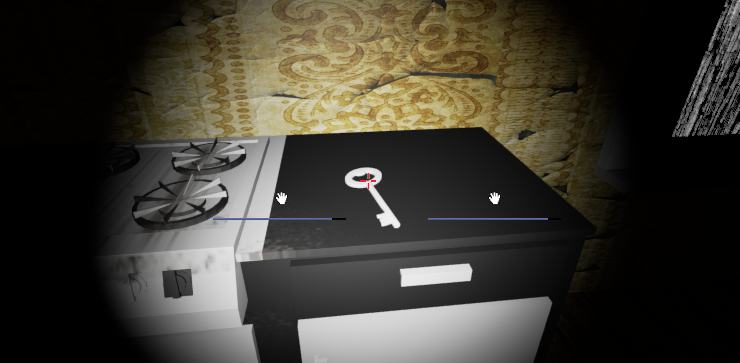
\includegraphics[scale=0.6]{ui1.png}
\caption{Progress bar of getting item}
\label{fig:ui1}
\end{figure}

\clearpage

The flowchart shows the logic of getting an item (Figure \ref{fig:ui2}). Event Dispatcher is used for the "look at" event.
\begin{figure}[h]
\centering
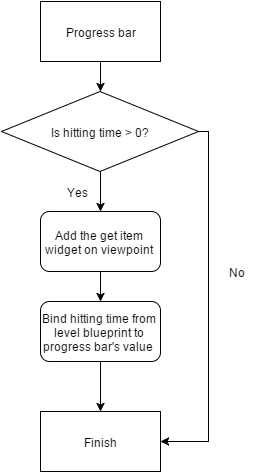
\includegraphics[scale=0.6]{ui2.png}
\caption{Flow chart on creating progress bar}
\label{fig:ui2}
\end{figure}

The function is called under event tick. That means the state of the progress bar is updated on every frame of the game play.

\subsection{Code quality}
To maintain a reusable environment, this project has done many re-factoring work. \\
The use of event dispatcher is one of the example. In the game there is a lot of item looking and getting events. There are many similarities between them. In Unreal Engine, we can create a class and event for look and get respectively. By binding the class to the item, it would call the look at event and save many repeated procedures.  

\clearpage

\section{Implementation}
\subsection{Challenges}

\begin{itemize}
  \item Story planning\\
  Game development is not just about coding, especially for horror game. The story planning is extremely important to a successful horror game. In addition, it is essential to find more natural ways to allow users to interact within a virtual environment.
  \item Use of game engine\\
  Getting start on new tools is always time consuming. As we spent a month on Google Cardboard with Unity, it took us quite a lot of time in spending on adapting Oculus SDK with Unreal Engine 4.
  \item VR Restrictions\\
  As VR game allow user to look around the scene, when we want to force the user to look at a certain event, it is essential to maintain the natural flow of the game. 
  \item Limited input\\
  To make the game more realistic, it is always better if the user can place the game with free hands. As a result, we need to take a lot of consideration when we want to give the control to user.
\end{itemize}

\subsection{Version Control}
Our project fully makes use of several tools for maintaining different versions of code.
\subsubsection{Git}
Git is widely used in open-source projects. Comparing to centralized version control system like Subversion, Git can store a local copy of the repository. It helps a lot when switching between commits and branches. It could take much time to re-download gigabytes of graphic assets from remote server. Branch in Git supports us developing experimental features without affecting and deleting previous bug-free versions. Branch merging is also fast and convenient. 

\subsubsection{GitHub}
GitHub is the most popular repository hosting website nowadays. GitHub provides a free hosting plan and an excellent user interface for tracing codes. One of GitHub functions heavily used in this project is issue management. We can record issues regarding enhancement or bugs on website and then closing or tagging them via commit message. Milestones for first semester is also set so that the project target is much clear and manageable.

\subsubsection{SourceTree}
SourceTree is a famous GUI application for Git and it is available on Mac OSX and Windows. SourceTree is good enough for novice of Git to visualize the branch tree and perform Git operation using buttons.

\subsubsection{Unreal Engine setting for Git}
In order to provide a smooth developing experience, Unreal Engine will pre-generate codes and shaders which may be 10 times larger than original asset size. Also, it is a good practice not to include compiled code so a gitignore file is formulated to guarantee that only source code is push to Git repository.

\clearpage

\section{Testing on user experience}
To make the game more terrifying and exciting, and also to test the players reactions, 15 classmates has invited to test the game.
\subsection{User Acceptance Test (UAT)}
\textbf{Problem spotted}
\begin{itemize}
\item The narration is not clear enough.\\
Some players said they cannot hear the narration sound very clearly. As a result, they found a hard time to get the instructions.
\item Many players find the key in corridor very fast.\\
They do not spend many time in corridor and miss some clues about the story. They can proceed to the lumber room directly
\item Some players get stuck in the game and do not know what should they do.\\
In lumber room, some players do not know they needed to look at the door to peek outside.
\item A few players found it hard to unlock the lumber room door.\\
They do not know they need to look at the key hole to open the door.
\end{itemize}
\textbf{Improvement made}
\begin{itemize}
\item Record the narration again and amplify the sound volume
\item Move the important item to a hidden place, so the player would spend more time to look at the scene.
\item Add narration in lumber room to give some hints to the player.
\item Increase the triggering area for the key hole in lumber door to make it easier to unlock the door.
\end{itemize}

\clearpage
\section{Limitation}
\begin{enumerate}
\item Screen resolution
The screen resolution of DK1 is not high enough to display clear text in stereo mode. It is hard for the player to read the on screen text and limited the ways to give instructions and story clues to the player.
\item Detecting Movement\\
Oculus Rift requires the connection with computer. This limited the user from big movement, e.g. walking and body rotating.
In addition, sensors in Oculus Rift Development Kit 1 is limited. This restricted the capture of movement from the player for more interactive function.

\end{enumerate}

\section{Future Development}

\subsection{Save game function}

Save all current status to a file and previous game progress can be able to retrieved when users choose to load a saved game. Current proposal is to divide the game into several stages and it can be called a "checkpoint". For example, the game currently can be divided into 3 stages (Living room, Corridor and Lumber room). As a result, we can formulate a subset of game status for each checkpoint instead of status of a whole game. 

We can pre-define a set of status for after passing each checkpoint. For example, if players can move from corridor to lumber room, they must get the key and open the door. So that it is guaranteed that both isKeyGot and isDoorOpened must be true. When loading the game process, we can apply the status so that we have the same status when users actually play the game.

\subsection{More clues of story}
The story is not completed in this stage. After getting out from lumber room, the player would get more clue about the murder with more events. The player would discover that Dora\textsc{\char13}s father is the murderer and he had killed Dora.

\subsection{Different endings due to player\textsc{\char13}s choice}
In a certain plot, the player can choose their choice in the game, which will lead to different endings.


\clearpage
\bibliographystyle{plain}
\bibliography{references}
\clearpage

\appendix
\begin{landscape}
\section{Gantt Chart for the project time line}
\begin{ganttchart}[
    canvas/.append style={fill=none, draw=black!5, line width=.75pt},
    hgrid style/.style={draw=black!5, line width=.75pt},
    vgrid={*1{draw=black!5, line width=.75pt}},
    today=13,
    today rule/.style={
      draw=black!64,
      dash pattern=on 3.5pt off 4.5pt,
      line width=1.5pt
    },
    today label font=\small\bfseries,
    title/.style={draw=none, fill=none},
    title label font=\bfseries\footnotesize,
    title label node/.append style={below=7pt},
    include title in canvas=false,
    bar label font=\mdseries\small\color{black!70},
    bar label node/.append style={left=2cm},
    bar/.append style={draw=none, fill=black!63},
    bar progress label font=\mdseries\footnotesize\color{black!70},
    group left shift=0,
    group right shift=0,
    group height=.5,
    group peaks tip position=0,
    group label node/.append style={left=.6cm},
    group progress label font=\bfseries\small,
    link/.style={-latex, line width=1.5pt},
    link label font=\scriptsize\bfseries,
    link label node/.append style={below left=-2pt and 0pt}
  ]{1}{13}
  \gantttitle[
    title label node/.append style={below left=7pt and -3pt}
  ]{WEEKS:\quad1}{1}
  \gantttitlelist{2,...,13}{1} \\
  \ganttgroup[progress=10]{Developing on Unity for Google Cardboard}{1}{5} \\
  \ganttbar[
  progress=70,
  name=cardboard
  ]{\textbf{1.1} Building Scene for living room}{1}{5} \\
  \ganttgroup{Developing on Unreal Engine 4 for Oculus}{5}{13}\\
  \ganttbar[progress=100]{\textbf{2.1} Scenes and events building for first three stages}{5}{12} \\
  \ganttbar[
    %progress=75,
    name=WBS1B
  ]{2.1.1 Living Room setting}{5}{8} \\
  \ganttbar[
    %progress=67,
    name=WBS1C
  ]{2.1.2 Corridor Setting}{7}{11} \\
  \ganttbar[
    %progress=50,
    name=WBS1D
  ]{2.1.3 Lumber Room Setting}{8}{11} \\
  \ganttbar[
    progress=100,
    name=WBS1E
  ]{\textbf{2.2} Testing and reviewing}{12}{13} \\[grid]
  \ganttlink[link type=f-s]{WBS1D}{WBS1E}
  \ganttlink[
    link type=f-f,
    link label node/.append style=left
  ]{WBS1C}{WBS1D}
\end{ganttchart}
\end{landscape}
\end{document}
